\documentclass[t]{beamer}
\usepackage{mathtools}
\usepackage{tikz}
\usepackage{pgfplots}
\usepackage{ulem}
\usetikzlibrary{arrows,backgrounds,shapes,matrix,positioning,fit}
\newcommand{\argmax}{\operatornamewithlimits{argmax}}
\newcommand{\argmin}{\operatornamewithlimits{argmin}}
\newcommand{\wt}{\operatornamewithlimits{wt}}
\newcommand{\var}{\operatornamewithlimits{var}}
\renewcommand\Re{\operatorname{Re}}
\renewcommand\Im{\operatorname{Im}}

\mode<presentation>
{
  \usetheme{Singapore}
  %\useoutertheme{infolines} % Showing only current section in navigation
  \setbeamertemplate{headline}{}  % Empty headline
  \setbeamertemplate{footline}[frame number]  % Getting rid of footer items except slide number
  \setbeamercovered{invisible}
  \beamertemplatenavigationsymbolsempty % Getting rid of navigation bullets at the bottom
}
\usepackage[english]{babel}
\usepackage[latin1]{inputenc}
\usepackage{times}
\usepackage[T1]{fontenc}

\title[EE 703 DMT]{Phase and Timing Synchronization}
\author[Saravanan V]
{
  Saravanan Vijayakumaran\\
  \href{mailto:sarva@ee.iitb.ac.in}{sarva@ee.iitb.ac.in}
}
\institute[IIT Bombay]
{
  Department of Electrical Engineering\\
  Indian Institute of Technology Bombay
}
\date{October 28, 2013}

\AtBeginSection[]%
{%
\begin{frame}[plain]%
  \topskip0pt
  \vspace*{\fill}
    \begin{center}%
      \usebeamerfont{section title}\insertsection%
    \end{center}%
  \vspace*{\fill}
\end{frame}%
}

\begin{document}

\begin{frame}
  \titlepage
\end{frame}

%% Frame %%
\begin{frame}{The System Model}
  \footnotesize
  \begin{itemize}
    \item \pause Consider the following complex baseband signal $s(t)$
      \begin{equation*}
        s(t) = \sum_{i=0}^{K-1} b_i p(t-iT)
      \end{equation*}
      where $b_i$'s are complex symbols
    \item \pause Suppose the LO frequency at the transmitter is $f_c$
      \begin{equation*}
        s_p(t) = \Re\left[\sqrt{2}s(t)e^{\ j2\pi f_c t}\right].
      \end{equation*}
    \item \pause Suppose that the LO frequency at the receiver is $f_c - \Delta f$
    \item \pause The received passband signal is
      \begin{equation*}
        y_p(t) = As_p(t-\tau) + n_p(t)
      \end{equation*}
    \item \pause The complex baseband representation of the received signal is then
      \begin{equation*}
        y(t) = Ae^{\ j(2\pi \Delta f t + \theta)}s(t-\tau) + n(t)
      \end{equation*}
  \end{itemize}
  \normalsize
\end{frame}

%% Frame %%
\begin{frame}{The System Model}
  \footnotesize
      \begin{equation*}
        y(t) = Ae^{\ j(2\pi \Delta f t + \theta)} \sum_{i=0}^{K-1} b_i p(t-iT-\tau) + n(t)
      \end{equation*}
  \begin{itemize}
    \item \pause The unknown parameters are $A$, $\tau$, $\theta$ and $\Delta f$
      \begin{description}
        \pause \item[Timing Synchronization] Estimation of $\tau$
        \pause \item[Carrier Synchronization] Estimation of $\theta$ and $\Delta f$
      \end{description}
    \item \pause The preamble of a packet contains known symbols called the training sequence
    \item \pause The $b_i$'s are known during the preamble
  \end{itemize}
  \normalsize
\end{frame}

%% Frame %%
\begin{frame}{Carrier Phase Estimation}
  \footnotesize
  \begin{itemize}
    \item The change in phase due to the carrier offset $\Delta f$ is $2\pi\Delta f T$ in a symbol interval $T$ 
    \item \pause The phase can be assumed to be constant over multiple symbol intervals
    \item \pause Assume that the phase $\theta$ is the only unknown parameter
    \item \pause Assume that $s(t)$ is a known signal in the following
      \begin{equation*}
        y(t) = s(t)e^{\ j\theta} + n(t)
      \end{equation*}
    \item \pause The likelihood function for this scenario is given by
      \begin{equation*}
        L(y|\theta) = \exp\left( \frac{1}{\sigma^2} \left[\Re(\langle y, s e^{\ j\theta}\rangle) - \frac{\lVert se^{\ j\theta} \rVert^2}{2} \right]\right)
      \end{equation*}
    \item \pause Let $\langle y, s \rangle = Z \pause = \lvert Z \rvert e^{\ j\phi} \pause = Z_c + jZ_s$
      \begin{eqnarray*}
        \pause \langle y, s e^{\ j\theta}\rangle & = & \pause e^{\ -j\theta}Z = \pause \lvert Z \rvert e^{\ j(\phi-\theta)} \\
        \pause \Re(\langle y, s e^{\ j\theta}\rangle) & = & \pause \lvert Z \rvert \cos (\phi-\theta)\\
        \pause \lVert se^{\ j\theta} \rVert^2  & = & \pause \lVert s \rVert^2
      \end{eqnarray*}
  \end{itemize} 
  \normalsize
\end{frame}

%% Frame %%
\begin{frame}{Carrier Phase Estimation}
  \footnotesize
  \begin{itemize}
    \item The likelihood function for this scenario is given by
      \begin{equation*}
        L(y|s_\theta) = \exp\left( \frac{1}{\sigma^2} \left[\lvert Z\rvert \cos (\phi -\theta) - \frac{\lVert s \rVert^2}{2} \right]\right)
      \end{equation*}
    \item \pause The ML estimate of $\theta$ is given by
      \begin{equation*}
        \hat{\theta}_{ML} = \pause \phi \pause = \arg(\langle y, s \rangle) \pause = \tan^{-1} \frac{Z_s}{Z_c}
      \end{equation*}
  \end{itemize} 
  \pause
  \begin{figure}
    \centering
      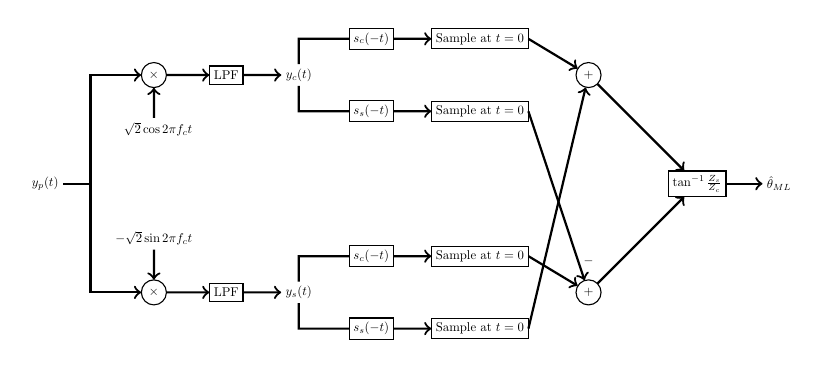
\begin{tikzpicture}[scale=0.46,transform shape]
        \node at (5,3) (yc) {$y_c(t)$};
        \node at (5,-3) (ys) {$y_s(t)$};
        \node[circle, draw, minimum size = 5mm] at (1,3) (prodc) {$\times$};
        \node[circle, draw, minimum size = 5mm] at (1,-3) (prods) {$\times$};
        \node[rectangle, draw, minimum size = 5mm] at (3,3) (LPc) {LPF};
        \node[rectangle, draw, minimum size = 5mm] at (3,-3) (LPs) {LPF};
        \node at (1,1.5) (cos) {$\ \ \sqrt{2}\cos 2\pi f_ct$};
        \node at (1,-1.5) (sin) {$-\sqrt{2}\sin 2\pi f_ct$};
        \node at (-2,0) (yp) {$y_p(t)$};
        \draw[->,thick] (prodc) -- (LPc);
        \draw[->,thick] (prods) -- (LPs);
        \draw[->,thick] (LPc) -- (yc);
        \draw[->,thick] (LPs) -- (ys);
        \draw[->,thick] (cos) -- (prodc);
        \draw[->,thick] (sin) -- (prods);
        \draw[->,thick] (-0.75,0) |- (prodc);
        \draw[->,thick] (-0.75,0) |- (prods);
        \draw[thick] (yp) -- (-0.75,0);
        \pause
        \node[rectangle, draw, minimum size = 5mm] at (7,4) (sc1) {$s_c(-t)$};
        \node[rectangle, draw, minimum size = 5mm] at (7,2) (ss1) {$s_s(-t)$};
        \node[rectangle, draw, minimum size = 5mm] at (7,-2) (sc2) {$s_c(-t)$};
        \node[rectangle, draw, minimum size = 5mm] at (7,-4) (ss2) {$s_s(-t)$};
        \node[rectangle, draw, minimum size = 5mm] at (10,4) (sampler1) {Sample at $t=0$};
        \node[rectangle, draw, minimum size = 5mm] at (10,2) (sampler2) {Sample at $t=0$};
        \node[rectangle, draw, minimum size = 5mm] at (10,-2) (sampler3) {Sample at $t=0$};
        \node[rectangle, draw, minimum size = 5mm] at (10,-4) (sampler4) {Sample at $t=0$};
        \draw[->,thick] (yc) |- (sc1) -- (sampler1);
        \draw[->,thick] (yc) |- (ss1) -- (sampler2);
        \draw[->,thick] (ys) |- (sc2) -- (sampler3);
        \draw[->,thick] (ys) |- (ss2) -- (sampler4);
        \pause
        \node[circle, draw, minimum size = 5mm] at (13, 3) (sum1) {$+$};
        \node[circle, draw, minimum size = 5mm] at (13, -3) (sum2) {$+$};
        \draw[->,thick] (sampler1.east) -- (sum1);
        \draw[->,thick] (sampler2.east) -- (sum2);
        \draw[->,thick] (sampler3.east) -- (sum2);
        \draw[->,thick] (sampler4.east) -- (sum1);
        \node[above=0.25cm of sum2] {$-$};
        \node[rectangle, draw, minimum size = 5mm] at (16,0) (tan) {$\tan^{-1} \frac{Z_s}{Z_c}$};
        \draw[->,thick] (sum1) -- (tan);
        \draw[->,thick] (sum2) -- (tan);
        \node[right=1cm of tan] (theta) {$\hat{\theta}_{ML}$};
        \draw[->,thick] (tan) -- (theta);
      \end{tikzpicture}
  \end{figure}
  \normalsize
\end{frame}

%% Frame %%
\begin{frame}{Phase Locked Loop}
  \footnotesize
  \begin{itemize}
    \item The carrier offset will cause the phase to change slowly
    \item \pause A tracking mechanism is required to track the changes in phase
    \item \pause For simplicity, consider an unmodulated carrier
      \begin{equation*}
        y_p(t) = \sqrt{2}\cos (2\pi f_c t + \theta(t)) + n_p(t)
      \end{equation*}
    \item \pause The complex baseband representation is
      \begin{equation*}
        y(t) = e^{\ j\theta(t)} + n(t)
      \end{equation*}
    \item \pause For an observation interval $T_o$, the log likelihood function is given by
      \begin{eqnarray*}
        \ln L(y|\theta) = \frac{1}{\sigma^2} \left[\Re\left(\langle y, e^{\ j\theta(t)}\rangle\right)- \frac{T_o}{2} \right]
      \end{eqnarray*}
    \item \pause  We get $\hat{\theta}_{ML}$ by maximizing
      \begin{equation*}
        J[\theta(t)] = \Re\left( \langle y, e^{\ j\theta(t)}\rangle\right) = \int_0^{T_o} \left[ y_c(t)\cos \theta(t) + y_s(t) \sin \theta(t) \right] \ dt
      \end{equation*}
  \end{itemize}
  \normalsize
\end{frame}

%% Frame %%
\begin{frame}{Phase Locked Loop}
  \footnotesize
  \begin{itemize}
    \item A necessary condition for a maximum at $\hat{\theta}_{ML}$ is 
      \begin{eqnarray*}
        \frac{\partial}{\partial \theta} J[\theta(t)] \bigg|_{\hat{\theta}_{ML}} = 0 \pause & \implies & \int_0^{T_o} \left[ -y_c(t)\sin \hat{\theta}_{ML} + y_s(t) \cos \hat{\theta}_{ML} \right] \ dt = 0 \\ \pause
                                                                                            & \implies & \Re\left(\langle y, je^{\ j\hat{\theta}_{ML}} \rangle \right) = 0 \\ \pause
                                                                                            & \implies & \langle y_p, -\sin (2\pi f_c t +\hat{\theta}_{ML}) \rangle = 0 \\ \pause
                                                                                            & \implies & -\int_{T_o} y_p(t) \sin (2\pi f_c t +\hat{\theta}_{ML}) \ dt = 0
      \end{eqnarray*}
    \pause
    \begin{figure}
      \centering
        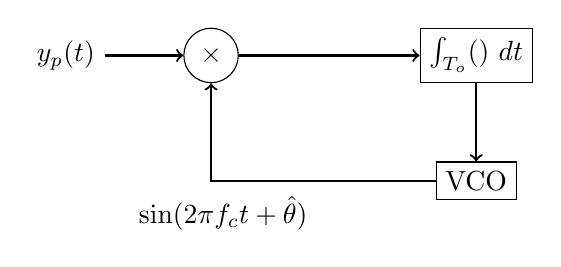
\begin{tikzpicture}[scale=1.0,transform shape]
          \node at (0,0) (yp) {$y_p(t)$};
          \node[draw, circle, right=1cm of yp] (prod) {$\times$};
          \node[draw, rectangle, right=4cm of yp] (int) {$\int_{T_o}() \ dt$};
          \node[draw, rectangle, below=1cm of int] (vco) {VCO};
          \draw[->,thick] (yp) -- (prod);
          \draw[->,thick] (prod) -- (int);
          \draw[->,thick] (int) -- (vco);
          \draw[->,thick] (vco.west) -| node[near start, below left=1mm] {$\sin (2\pi f_c t + \hat{\theta})$}  (prod);
        \end{tikzpicture}
    \end{figure}
  \end{itemize}
  \normalsize
\end{frame}

%% Frame %%
\begin{frame}{Symbol Timing Estimation}
  \footnotesize
  \begin{itemize}
    \item Consider the complex baseband received signal 
      \begin{equation*}
        y(t) = As(t-\tau)e^{\ j\theta} + n(t)
      \end{equation*}
      where $A$, $\tau$ and $\theta$ are unknown and $s(t)$ is known
    \item \pause For $\gamma = [\tau, \theta, A]$ and $s_\gamma(t) = As(t-\tau)e^{\ j\theta}$, the likelihood function is
      \begin{equation*}
        L(y|\gamma) = \exp\left( \frac{1}{\sigma^2} \left[\Re\left(\langle y, s_\gamma\rangle\right) - \frac{\lVert s_\gamma \rVert^2}{2} \right]\right)
      \end{equation*}
    \item \pause For a large enough observation interval, the signal energy does not depend on $\tau$ \pause and $\lVert s_\gamma \rVert^2 = A^2\lVert s \rVert^2$
    \item \pause For $s_{MF}(t) = s^*(-t)$ we have 
      \begin{eqnarray*}
        \langle y, s_\gamma \rangle & = & Ae^{\ -j\theta} \int y(t) s^*(t-\tau) \ dt \\ \pause
                                    & = & \pause A e^{\ -j\theta}\int y(t) s_{MF}(\tau -t) \ dt \\ \pause
                                    & = & Ae^{\ -j\theta} (y\star s_{MF})(\tau)
      \end{eqnarray*}
  \end{itemize}
  \normalsize
\end{frame}

%% Frame %%
\begin{frame}{Symbol Timing Estimation}
  \footnotesize
  \begin{itemize}
    \item Maximizing the likelihood function is equivalent to maximizing the following cost function
      \begin{equation*}
        J(\tau, A, \theta) = \Re\left( Ae^{\ -j\theta}(y\star s_{MF})(\tau)\right) - \frac{A^2 \lVert s \rVert^2}{2}
      \end{equation*}
    \item \pause For $(y\star s_{MF})(\tau) = Z(\tau) = \lvert Z(\tau) \rvert e^{\ j\phi(\tau)}$ we have
      \begin{equation*}
        \Re\left( Ae^{\ -j\theta} (y\star s_{MF})(\tau)\right)  = A \lvert Z(\tau) \rvert \cos(\phi(\tau) - \theta)
      \end{equation*}
    \item \pause The maximizing value of $\theta$ is equal to $\phi(\tau)$
    \item \pause Substituting this value of $\theta$ gives us the following cost function
      \begin{equation*}
        J(\tau, A) = \argmax_{\theta} J(\tau, A, \theta) = A\lvert (y\star s_{MF})(\tau)\rvert - \frac{A^2 \lVert s \rVert^2}{2}
      \end{equation*}
  \end{itemize}
  \normalsize
\end{frame}

%% Frame %%
\begin{frame}{Symbol Timing Estimation}
  \footnotesize
  \begin{itemize}
    \item The ML estimator of the delay picks the peak of the matched filter output
      \begin{equation*}
        \hat{\tau}_{ML} = \argmax_\tau \lvert (y\star s_{MF})(\tau) \rvert
      \end{equation*}
  \end{itemize}
  \pause
  \begin{figure}
    \centering
      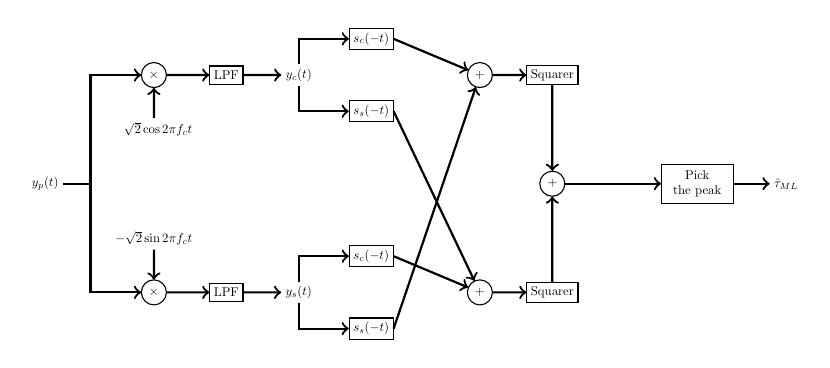
\begin{tikzpicture}[scale=0.46,transform shape]
        \node at (5,3) (yc) {$y_c(t)$};
        \node at (5,-3) (ys) {$y_s(t)$};
        \node[circle, draw, minimum size = 5mm] at (1,3) (prodc) {$\times$};
        \node[circle, draw, minimum size = 5mm] at (1,-3) (prods) {$\times$};
        \node[rectangle, draw, minimum size = 5mm] at (3,3) (LPc) {LPF};
        \node[rectangle, draw, minimum size = 5mm] at (3,-3) (LPs) {LPF};
        \node at (1,1.5) (cos) {$\ \ \sqrt{2}\cos 2\pi f_ct$};
        \node at (1,-1.5) (sin) {$-\sqrt{2}\sin 2\pi f_ct$};
        \node at (-2,0) (yp) {$y_p(t)$};
        \draw[->,thick] (prodc) -- (LPc);
        \draw[->,thick] (prods) -- (LPs);
        \draw[->,thick] (LPc) -- (yc);
        \draw[->,thick] (LPs) -- (ys);
        \draw[->,thick] (cos) -- (prodc);
        \draw[->,thick] (sin) -- (prods);
        \draw[->,thick] (-0.75,0) |- (prodc);
        \draw[->,thick] (-0.75,0) |- (prods);
        \draw[thick] (yp) -- (-0.75,0);
        \node[rectangle, draw, minimum size = 5mm] at (7,4) (sc1) {$s_c(-t)$};
        \node[rectangle, draw, minimum size = 5mm] at (7,2) (ss1) {$s_s(-t)$};
        \node[rectangle, draw, minimum size = 5mm] at (7,-2) (sc2) {$s_c(-t)$};
        \node[rectangle, draw, minimum size = 5mm] at (7,-4) (ss2) {$s_s(-t)$};
        \draw[->,thick] (yc) |- (sc1);
        \draw[->,thick] (yc) |- (ss1);
        \draw[->,thick] (ys) |- (sc2);
        \draw[->,thick] (ys) |- (ss2);
        \node[circle, draw, minimum size = 5mm] at (10, 3) (sum1) {$+$};
        \node[circle, draw, minimum size = 5mm] at (10, -3) (sum2) {$+$};
        \draw[->,thick] (sc1.east) -- (sum1);
        \draw[->,thick] (ss1.east) -- (sum2);
        \draw[->,thick] (sc2.east) -- (sum2);
        \draw[->,thick] (ss2.east) -- (sum1);
        \node[rectangle, draw, minimum size = 5mm] at (12, 3) (squarer1) {Squarer};
        \node[rectangle, draw, minimum size = 5mm] at (12, -3) (squarer2) {Squarer};
        \node[circle, draw] at (12, 0) (summer) {$+$};
        \draw[->,thick] (sum1) -- (squarer1);
        \draw[->,thick] (sum2) -- (squarer2);
        \draw[->,thick] (squarer1) -- (summer);
        \draw[->,thick] (squarer2) -- (summer);
        \node[rectangle, draw, minimum size = 5mm] at (16,0) (peakpicker) {\begin{tabular}{c} Pick \\ the peak \end{tabular}};
        \draw[->,thick] (summer) -- (peakpicker);
        \node[right=1cm of peakpicker] (tau) {$\hat{\tau}_{ML}$};
        \draw[->,thick] (peakpicker) -- (tau);
      \end{tikzpicture}
  \end{figure}
  \normalsize
\end{frame}

%% Frame %%
\begin{frame}{Early-Late Gate Synchronizer}
  \footnotesize
  \begin{itemize}
    \item Timing tracker which exploits symmetry in matched filter output \pause
      \begin{columns}
        \begin{column}{0.5\textwidth}
        \begin{figure}
          \centering
            \begin{tikzpicture}[scale=0.6,transform shape]
              \begin{axis}[
                           title=$p(t)$,
                           xmax=3.5,
                           xmin=0,
                           ymax=1.5,
                           ymin=0,
                           axis lines = left,
                           ytick={1,0},
                           xtick = {0,1.5,3.5},
                           xticklabels = {$0$,$T$,$t$},
                           yticklabels = {1},
                          ]
                \addplot[color=blue,very thick] coordinates {(0,1) (1.5,1) (1.5,0)};
              \end{axis}
            \end{tikzpicture}
        \end{figure}
      \end{column}

    \pause
      \begin{column}{0.5\textwidth}
        \begin{figure}
          \centering
            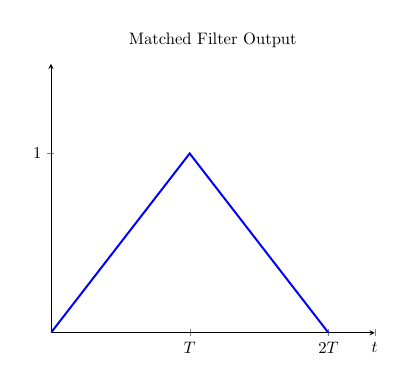
\begin{tikzpicture}[scale=0.6,transform shape]
              \begin{axis}[
                           title={Matched Filter Output},
                           xmax=3.5,
                           xmin=0,
                           ymax=1.5,
                           ymin=0,
                           axis lines = middle,
                           ytick={1},
                           xtick = {0,1.5,3,3.5},
                           xticklabels = {$0$,$T$,$2T$,$t$},
                           yticklabels = {1},
                          ]
                \addplot[color=blue,very thick] coordinates {(0,0) (1.5,1) (3,0)};
              \end{axis}
            \end{tikzpicture}
        \end{figure}
        \end{column}
      \end{columns}
  \end{itemize}
  \normalsize
\end{frame}

%% Frame %%
\begin{frame}{Early-Late Gate Synchronizer}
  \footnotesize
  \begin{figure}
    \centering
      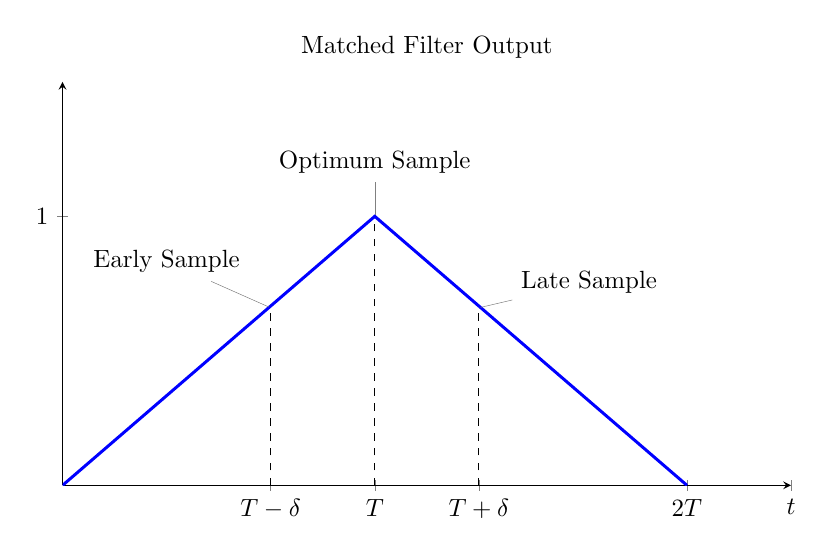
\begin{tikzpicture}[scale=0.9,transform shape]
        \begin{axis}[
                     title={Matched Filter Output},
                     xmax=3.5,
                     xmin=0,
                     ymax=1.5,
                     ymin=0,
                     axis lines = middle,
                     ytick={1},
                     xtick = {0,1,1.5,2,3,3.5},
                     xticklabels = {$0$,$T-\delta$,$T$,$T+\delta$,$2T$,$t$},
                     yticklabels = {1},
                     x post scale = 1.5
                    ]
          \addplot[color=blue,very thick] coordinates {(0,0) (1.5,1) (3,0)};
          \draw[dashed] (axis cs:1.5,0) -- (axis cs:1.5,1);
          \node at (axis cs:1.5,1) [pin={Optimum Sample},inner sep=0pt] {};
          \draw[dashed] (axis cs:1,0) -- (axis cs:1,0.66);
          \node at (axis cs:1,0.66) [pin={130:Early Sample},inner sep=0pt] {};
          \draw[dashed] (axis cs:2,0) -- (axis cs:2,0.66);
          \node at (axis cs:2,0.66) [pin={10:Late Sample},inner sep=0pt] {};
        \end{axis}
      \end{tikzpicture}
  \end{figure}
  \begin{itemize}
    \item \pause The values of the early and late samples are equal
  \end{itemize}
  \normalsize
\end{frame}

%% Frame %%
\begin{frame}{Early-Late Gate Synchronizer}
  \footnotesize
  \begin{figure}
    \centering
      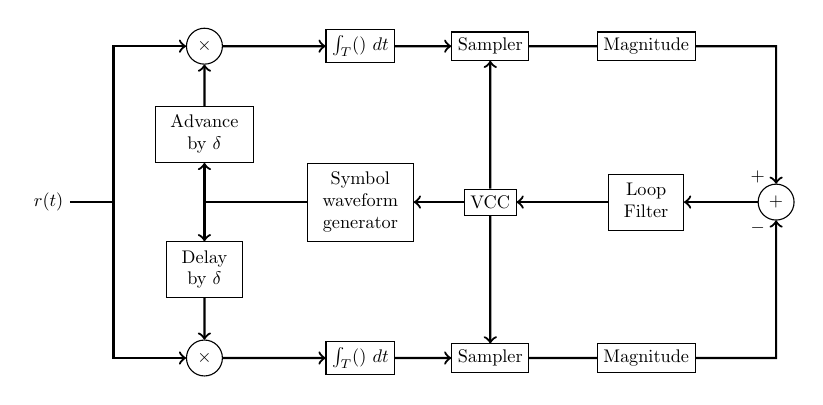
\begin{tikzpicture}[scale=0.66,transform shape]
        \node[circle, draw, minimum size = 5mm] at (1,3) (prodc) {$\times$};
        \node[circle, draw, minimum size = 5mm] at (1,-3) (prods) {$\times$};
        \node[rectangle, draw, minimum size = 5mm] at (4,3) (intc) {$\int_T () \ dt$};
        \node[rectangle, draw, minimum size = 5mm] at (4,-3) (ints) {$\int_T () \ dt$};
        \node[rectangle, draw, minimum size = 5mm] at (1,1.3) (adv) {$\begin{array}{c} \text{Advance} \\ \text{by } \delta \end{array}$};
        \node[rectangle, draw, minimum size = 5mm] at (1,-1.3) (del) {$\begin{array}{c} \text{Delay} \\ \text{by } \delta \end{array}$};
        \node at (-2,0) (rt) {$r(t)$};
        \draw[->,thick] (prodc) -- (intc);
        \draw[->,thick] (prods) -- (ints);
        \draw[->,thick] (adv) -- (prodc);
        \draw[->,thick] (del) -- (prods);
        \draw[->,thick] (-0.75,0) |- (prodc);
        \draw[->,thick] (-0.75,0) |- (prods);
        \draw[thick] (rt) -- (-0.75,0);
        \node[rectangle, draw, minimum size = 5mm] at (6.5,3) (samplerc) {Sampler};
        \node[rectangle, draw, minimum size = 5mm] at (6.5,-3) (samplers) {Sampler};
        \node[rectangle, draw, minimum size = 5mm] at (9.5,3) (magc) {Magnitude};
        \node[rectangle, draw, minimum size = 5mm] at (9.5,-3) (mags) {Magnitude};
        \node[rectangle, draw, minimum size = 5mm] at (9.5,0) (loopf) {$\begin{array}{c} \text{Loop} \\ \text{Filter}\end{array}$};
        \node[rectangle, draw, minimum size = 5mm] at (6.5,0) (vcc) {VCC};
        \node[rectangle, draw, minimum size = 5mm] at (4,0) (symbgen) {$\begin{array}{c} \text{Symbol} \\ \text{waveform} \\ \text{generator} \end{array}$};
        \draw[->,thick] (intc) -- (samplerc);
        \draw[->,thick] (ints) -- (samplers);
        \node[circle, draw, minimum size = 5mm] at (12,0) (sum) {$+$};
        \node[above=0.25cm of sum.west] {$+$};
        \node[below=0.25cm of sum.west] {$-$};
        \draw[->,thick] (samplerc) -- (magc) -| (sum);
        \draw[->,thick] (samplers) -- (mags) -| (sum);
        \draw[->,thick] (sum) -- (loopf);
        \draw[->,thick] (loopf) -- (vcc);
        \draw[->,thick] (vcc) -- (symbgen);
        \draw[->,thick] (symbgen) -| (del);
        \draw[->,thick] (symbgen) -| (adv);
        \draw[->,thick] (vcc.south) -- (samplers);
        \draw[->,thick] (vcc.north) -- (samplerc);
      \end{tikzpicture}
  \end{figure}
  \begin{itemize}
    \item \pause The motivation for this structure can be seen from the following approximation
    \begin{equation*}
      \frac{dJ(\tau)}{d\tau} \approx \frac{J(\tau +\delta) - J(\tau - \delta)}{2\delta}
    \end{equation*}
  \end{itemize}
  \normalsize
\end{frame}

%% Frame %%
\begin{frame}{}
\vfill
\begin{center}
Thanks for your attention
\end{center}
\vfill
\end{frame}

\end{document}
